\section{Wer ist also JS, und wer diese Jutta Schell?}
\begin{wrapfigure}{r}{0.5\textwidth}\centering \vspace{-10pt}
    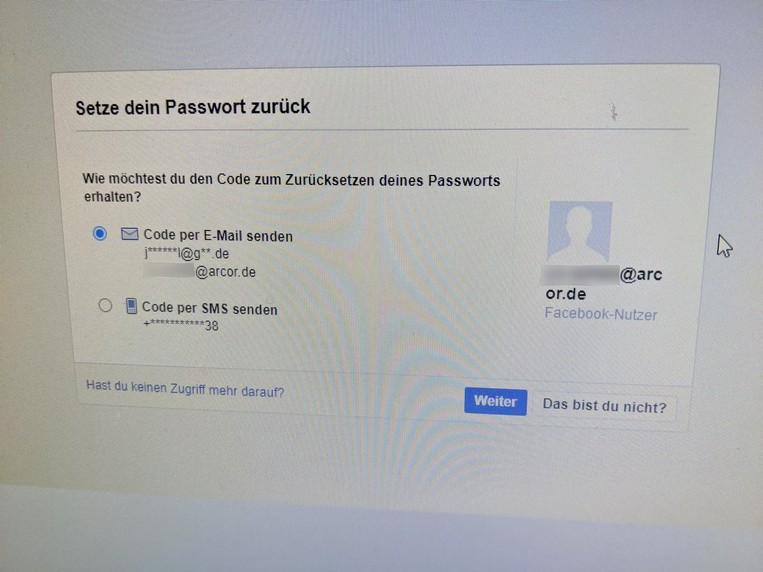
\includegraphics[width=0.4\textwidth]{images/image--007.jpg}
    \caption{}\label{image:7} \vspace{-20pt}
\end{wrapfigure}
Die Recherche ist schnell gemacht. Laut ihrem Profil bei
Xing \autocite{8} ist Jutta studierte Rechtswissenschaftlerin. Sie hat
von 1991-1999 in Heidelberg studiert.  Bei Facebook haben wir nach ihr gesucht, aber nur ein deaktiviertes Profil \autocite{9} \autocite{10} gefunden, das aber mit ihrer Mailadresse und Handynummer registriert ist (siehe \cref{image:7}). Die Daten führen wiederum auf ihre Homepage (siehe \cref{image:11}). Sie züchtet auch Kaninchen \autocite{11} und ist Mitglied in der Arbeitsgemeinschaft der Widderzüchter im ZDRK \autocite{12}. Aber deswegen machen wir uns keine Sorgen.
\begin{figure}[hbt!]\centering
  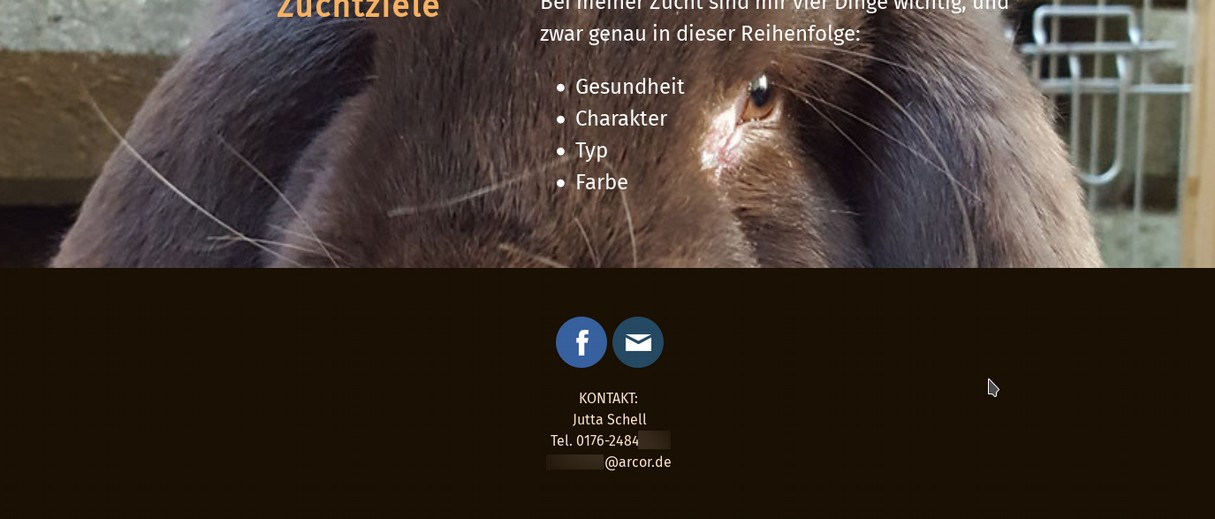
\includegraphics[width=0.6\textwidth]{images/image--011.jpg}
  \caption{}
  \label{image:11}
\end{figure}

Eine der Regeln von Jutta Schell lautet:  „Keine Hassbotschaften: Hetze und Gewaltbotschaften sind nicht erwünscht.“ Aber der Chat ist voll davon. Davon und von Theorien über – nun, so allerlei (siehe \cref{image:10,image:8,image:9}).
\begin{figure}[hbt!]\centering
  \subfloat[]{
    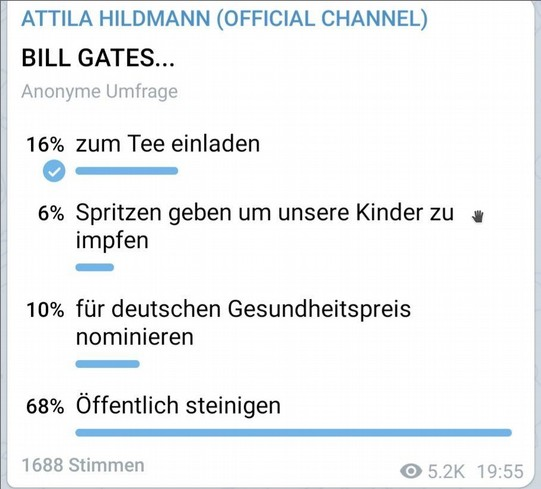
\includegraphics[width=0.3\textwidth]{images/image--010.jpg}
    \label{image:10}
  }
  \subfloat[]{
    
\includegraphics[width=.35\textwidth]{images/image--008.png}
    \label{image:8}
  }
  \subfloat[]{
    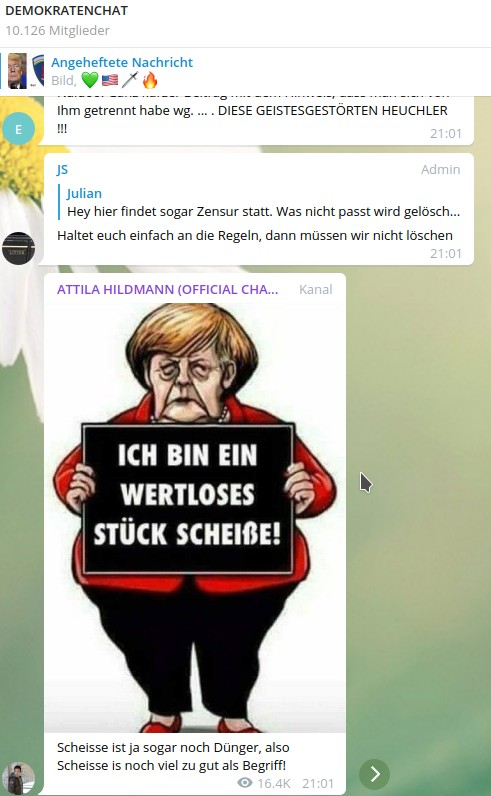
\includegraphics[width=.3\textwidth]{images/image--009.jpg}
    \label{image:9}
  }
  \caption{}
\end{figure}

Und wir könnten noch mehr Beispiele liefern, denn gelöscht wird nur, was nicht in die absurde Welt des Attila Hildmann und seiner Telegram-Blase passt. Aber vielleicht wäre es einfacher, den DEMOKRATENCHAT einfach selbst zu verfolgen \dots oder Frau Schell zu fragen.

\begin{wrapfigure}{r}{0.35\textwidth}\centering  \vspace{-10pt}
  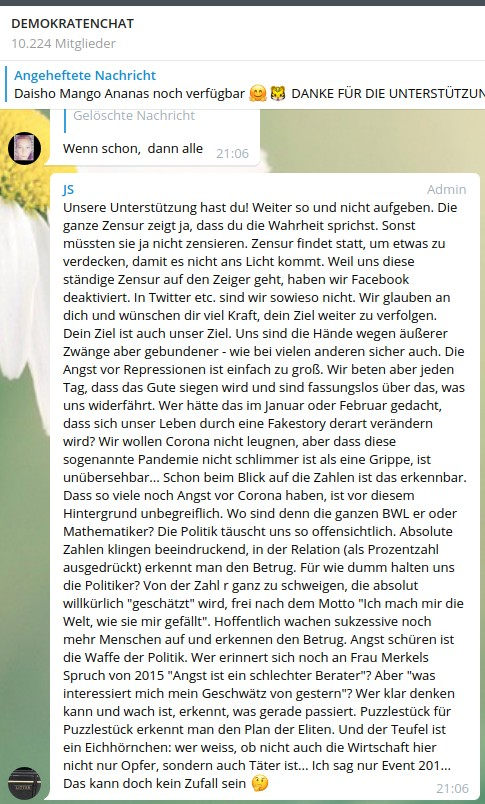
\includegraphics[width=0.4\textwidth]{images/image--012.jpg}
  \caption{}\label{image:12}\vspace{-24pt}
\end{wrapfigure}
„Unsere Unterstützung hast du! Weiter so und nicht aufgeben. Die ganze Zensur zeigt ja, dass du die Wahrheit sprichst. Sonst müssten sie ja nicht zensieren. Zensur findet statt, um etwas zu verdecken, damit es nicht ans Licht kommt. Weil uns diese ständige Zensur auf den Zeiger geht, haben wir Facebook deaktiviert. In Twitter etc. sind wir sowieso nicht. Wir glauben an dich und wünschen dir viel Kraft, dein Ziel  weiter zu verfolgen. Dein Ziel ist auch unser Ziel. Uns sind die Hände wegen äußerer Zwänge aber gebundener - wie bei vielen anderen sicher auch.\newline
[\dots]\newline
Wer klar denken kann und wach ist, erkennt, was gerade passiert. Puzzlestück für  Puzzlestück erkennt man den Plan der Eliten. Und der Teufel ist ein Eichhörnchen:  wer weiss, ob nicht auch die Wirtschaft hier nicht nur Opfer, sondern auch Täter ist\dots Ich sag nur Event 201\dots Das kann doch kein Zufall sein“\autocite{13}
% \captionof{floatquote}{JS in DEMOKRATENCHAT}\label{quo:11}
